% !TeX root = ../ejemplo.tex

\section{Códigos QR}

Para la elaboración de nuestro TT, el código QR desempeña un papel fundamental en la corroboración de la identidad de los estudiantes. Las credenciales escolares al contener un código QR se puede aprovechar la capacidad para almacenar y transmitir información de manera segura y rápida. Este enfoque nos permite verificar la información del estudiante mediante un simple escaneo, reduciendo el tiempo necesario para corroborar la identidad. Al escanear el código QR en la credencial. El sistema accede a los datos del alumno, lo cual permite verificar si coincide con la persona que se presenta al ETS.

Un código QR es un tipo de código de barras bidimensionales que solo se puede leer con teléfonos inteligentes u otros dispositivos dedicados a la lectura de estos códigos. Cuando se lee un código QR, los dispositivos se conectan directamente a mensajes de texto, correos electrónicos, sitios web, números de teléfono, etc \cite{CitaA01}.

\subsection{Anatomía de un código QR}
\title{Patrones de detección de posición}\\

\begin{figure}[htbp]
	\begin{center}
		\fbox{
\includegraphics[width=.24\textwidth]{images/img01}}
		\caption{Patrones de detección de posición.}
		\label{fig:Patrones de deteccion de posicion2}
	\end{center}
\end{figure}

Los patrones de detección de posición se encuentran en las tres esquinas del código. Gracias a ellos, el escáner puede reconocer y leer el código QR rápidamente. Estos marcadores indican la dirección en la que se imprimió el código QR y ayudan a su identificación y orientación. \\

\title{Patrones de alineación}

\begin{figure}[htbp]
	\begin{center}
		\fbox{
\includegraphics[width=.24\textwidth]{images/img02}}
		\caption{Patrones de alineación.}
		\label{fig:Patrones de alineacion1}
	\end{center}
\end{figure}

Usados para corregir la distorsión del código QR en superficies curvas. El tamaño y la cantidad de los patrones de alineación pueden variar según el volumen de la información almacenada en el código \cite{CitaA01}. \\

\title{Patrones de temporización}

\begin{figure}[htbp]
	\begin{center}
		\fbox{
\includegraphics[width=.24\textwidth]{images/img03}}
		\caption{Patrones de temporización.}
		\label{fig:temporizacion}
	\end{center}
\end{figure}

La alternancia de los módulos negros y blancos del código QR detrmina el sistema de información, también llamado cuadrícula de datos. Con estas líneas, el escáner reconoce la matriz de datos. 

\newpage

\title{Información sobre la versión}

\begin{figure}[htbp]
	\begin{center}
		\fbox{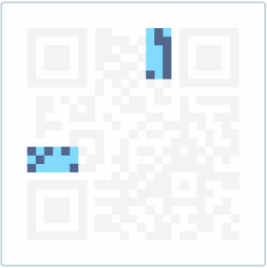
\includegraphics[width=.24\textwidth]{images/img04}}
		\caption{Información sobre la versión.}
		\label{fig:version}
	\end{center}
\end{figure}

Estos marcadores indican cuál de las 40 versiones del código QR está siendo usada. Normalmente las versiones utilizadas son de 1 a 7. \cite{CitaA01}\\

\title{Información del formato}

\begin{figure}[htbp]
	\begin{center}
		\fbox{
\includegraphics[width=.24\textwidth]{images/img05}}
		\caption{Información del formato.}
		\label{fig:formato2}
	\end{center}
\end{figure}

Contiene información sobre la tolerancia a los errores y el patrón del enmascaramiento de datos. La información sobre el formato facilita el escaneo del código. \cite{CitaA01}\\

\newpage
\title{Código de corrección de datos y errores}

\begin{figure}[htbp]
	\begin{center}
		\fbox{
\includegraphics[width=.24\textwidth]{images/img06}}
		\caption{Código de corrección de datos y errores.}
		\label{fig:erroresDatos}
	\end{center}
\end{figure}

El sistema de corrección de errores del código QR almacena toda la información y comparte el espacio con los módulos de corrección de errores, que permiten reconstruir los datos perdidos\cite{CitaA01} . \\

\title{Márgenes}

\begin{figure}[htbp]
	\begin{center}
		\fbox{
\includegraphics[width=.24\textwidth]{images/img07}}
		\caption{Márgenes.}
		\label{fig:margenes}
	\end{center}
\end{figure}

Los márgenes, o también llamado zona quieta, alrededor del código QR son similares al espacio blanco en un diseño, proporcionan estructura y una mejor comprensión. Pero, ¿cómo? Para que el software de escaneo identifique bien el límite del código QR de sus alrededores, los márgenes son vitales.

\subsection{Fiabilidad de los códigos QR}
Los códigos QR están diseñados para mantener la información legible, aunque estén oscuros o dañados. Esto se logra mediante la compensación de errores, es decir, insertando la información varias veces. Con un alto nivel de seguridad, los códigos QR pueden leerse incluso si un tercio de su información es ilegible. Esto hace que los códigos QR sean muy fiables a la hora de guardar información. \\

